\documentclass[a4paper, 12pt]{article}

\usepackage[portuges]{babel}
\usepackage[utf8]{inputenc}
\usepackage{amsmath, amsthm,amssymb}
\usepackage{indentfirst}
\usepackage{graphicx}
\usepackage{url}
\usepackage{float}
\usepackage{subcaption}

\newtheorem{defin}{Definição}[section]
\newtheorem{obs}{Observação}[section]
\newtheorem{teo}{Teorema}[section]
\newtheorem{nota}{Nota}[section]
\newtheorem{lema}{Lema}[section]



%Python code

\usepackage{listings}
\usepackage{xcolor}
\definecolor{codegreen}{rgb}{0,0.6,0}
\definecolor{codegray}{rgb}{0.5,0.5,0.5}
\definecolor{codepurple}{rgb}{0.58,0,0.82}
\definecolor{backcolour}{rgb}{0.95,0.95,0.92}

\lstdefinestyle{mystyle}{
	backgroundcolor=\color{backcolour},   
	commentstyle=\color{codegreen},
	keywordstyle=\color{magenta},
	numberstyle=\tiny\color{codegray},
	stringstyle=\color{codepurple},
	basicstyle=\ttfamily\footnotesize,
	breakatwhitespace=false,         
	breaklines=true,                 
	captionpos=b,                    
	keepspaces=true,                 
	numbers=left,                    
	numbersep=5pt,                  
	showspaces=false,                
	showstringspaces=false,
	showtabs=false,                  
	tabsize=2
}

\lstset{style=mystyle}


\setlength{\unitlength}{1cm}
\thicklines

\begin{document}

\begin{titlepage}
	\begin{center}
		
		\begin{figure}[!htb]
			\centering
			
\includegraphics[width=5cm]{uminho}
			\label{Rotulo}
		\end{figure}
		%\vspace{1cm}
		
		\textbf{\Huge{Universidade do Minho}}\\
		\vspace{10pt}
		\large{Escola de Ciências da Universidade do Minho}\\
		\large{Departamento de Informática}\\
		\vspace{10pt}
		\normalsize{Mestrado em Matemática e Computação}\\
		\normalsize{Mestrado Integrado em Engenharia Informática}\\
		\vspace{2cm}
		\textbf{\Large{Redes Neuronais Recorrentes para previsão do fluxo de tráfego rodoviário}}\\
		\vspace{2cm}
	\end{center}
	
	\begin{center}
		\textbf{Alunos:}
		\vspace{0,1cm}
		\\Andreia Costa (PG37013) \\Henrique Faria (A82200) \\ Paulo Barbosa (PG40160) \\ Rui Teixeira (PG37021)\\
		\vspace{1cm}
		\textbf{Docentes:} \\
		Bruno Fernandes\\ 
		Victor Alves \\
		\vspace{1cm}
		\textbf{Unidade Curricular:} Classificadores e Sistemas Conexionistas
	\end{center}
	\vspace{1cm}
	\begin{center}
		Maio\\
		2020
	\end{center}
\end{titlepage}

\newpage
% % % % % % % % % % % % % % % % % % % % % % % % % %
\newpage
\tableofcontents
\thispagestyle{empty}

\newpage
\pagenumbering{arabic}

\section{Introdução}


\newpage

\section{\textit{Dataset}}

Aquando da apresentação do presente trabalho foram disponibilizados dados referentes a duas cidades: Braga e Porto, sendo que o grupo escolheu os dados relativos à cidade de Braga para trabalhar.

Os dados encontram-se distribuídos em $4$ \textit{datasets}:

\begin{itemize}
	\item \textit{Traffic Flow Braga Until 20191231};
	\item \textit{Traffic Incidents Braga Until 20191231};
	\item \textit{Weather Braga Descriptions Until 20191231};
	\item \textit{Weather Braga Until 20191231}.
\end{itemize}

Todos os \textit{datasets} contêm dados relativos ao período entre $15$ Janeiro $2019$ e $31$ Dezembro $2019$.

\subsection{\textit{Traffic Flow Braga}}

O \textit{dataset "Traffic Flow Braga" } é constituído pelos seguintes atributos:

\begin{itemize}
	\item $city\_name$;
	\item $road\_num$;
	\item $road\_name$;
	\item $functional\_road\_class\_desc$;
	\item $current\_speed$;
	\item $free\_flow\_speed$;
	\item $speed\_diff$;
	\item $current\_travel\_time$;
	\item $free_flow\_travel\_time$;
	\item $time\_diff$;
	\item $creation\_date$.
\end{itemize}

\subsection{\textit{Traffic Incidents Braga}}

\begin{itemize}
	\item $city\_name$;
	\item $description$;
	\item $cause\_of\_incident$;
	\item $from\_road$;
	\item $to\_road$;
	\item $affected\_roads$;
	\item $incident\_category\_desc$;
	\item $magnitude\_of\_delay\_desc$;
	\item $length\_in\_meters$;
	\item $delay\_in\_seconds$;
	\item $incident\_date$;
	\item $latitude$;
	\item $longitude$.
\end{itemize}

\subsection{\textit{Weather Braga Descriptions}}

\begin{itemize}
	\item $city\_name$;
	\item $cloudiness$;
	\item $atmosphere$;
	\item $snow$;
	\item $thunderstorm$;
	\item $rain$;
	\item $sunrise$;
	\item $sunset$;
	\item $creation\_date$.
\end{itemize}

\subsection{\textit{Weather Braga}}

\begin{itemize}
	\item $city\_name$;
	\item $temperature$;
	\item $atmospheric\_pressure$;
	\item $humidity$;
	\item $wind\_speed$;
	\item $clouds$;
	\item $precipitation$;
	\item $current\_luminosity$;
	\item $sunrise$;
	\item $sunset$;
	\item $creation\_date$.
\end{itemize}

\subsection{Preparação dos dados}

Após análise dos quatro \textit{datasets} concluiu-se que, antes de se desenvolver o modelo para a previsão da \textit{feature speed\_diff}, era necessário fazer uma prévia preparação dos dados.

Começou-se por fazer um prévio tratamento do \textit{dataset Traffic\_Incidents}. Para isso, quadriplicou-se esse \textit{dataset}, com o intuito de atribuir todas as ruas em estudo a todos os incidentes, para que posteriormente fosse possível avaliar a distância entre os incidentes e as ruas em estudo. 

\begin{figure}[H]
	\centering
	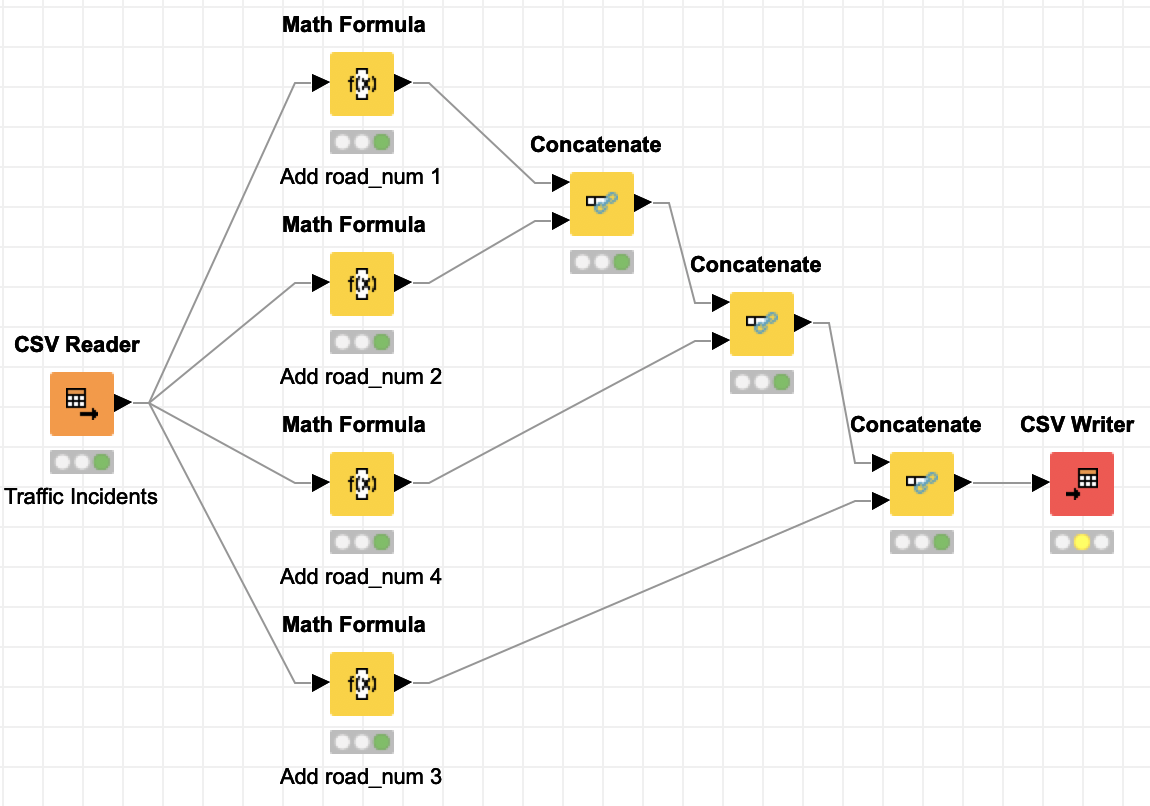
\includegraphics[width=10cm]{Traffic_Incidents}
	\caption{Preparação do \textit{dataset Traffic\_Incidentes}.}
\end{figure}

De seguida, recorrendo à latitude e longitude dos diferentes acontecimentos, calculou-se a distância dos incidentes a cada uma das ruas, para perceber quais os incidentes que podiam influenciar o \textit{speed\_diff} de uma determinada rua.

\begin{lstlisting}[language=Python]
import pandas as pd
from math import radians, sin, cos, atan2, sqrt

df = pd.read_csv('Traffic_Incidents.csv', delimiter = ',', error_bad_lines = False, encoding = 'ISO-8859-1')

def distance(p1, n):
	R = 6371.0
	if n == 1:
	lat2 = radians(41.548331)
	lon2 = radians(-8.421298)
	elif n == 2:
	lat2 = radians(41.551356)
	lon2 = radians(-8.420001)
	elif n == 3:
	lat2 = radians(41.546639)
	lon2 = radians(-8.433517)
	else:
	lat2 = radians(41.508849)
	lon2 = radians(-8.462299)
	lat1, lon1 = radians(p1[0]), radians(p1[1])
	dlon = lon2 - lon1
	dlat = lat2 - lat1
	a = sin(dlat / 2)**2 + cos(lat1) * cos(lat2) * sin(dlon / 2)**2
	c = 2 * atan2(sqrt(a), sqrt(1 - a))
	distance = R * c
return distance

df['Distance'] = df.apply(lambda row: distance((row['latitude'],row['longitude']), row['road_num']), axis=1)
\end{lstlisting}

Após calculadas todas as distâncias fez-se um tratamento estatístico, tendo-se obtido os seguintes resultados:

\begin{itemize}
	\item ${max}= 6313,251$;
	\item ${min}= 0,0228$;
	\item ${mean}= 4,507$;
	\item ${standard \ deviation}= 81,789$.
\end{itemize}

Através dos resultados obtidos é possível verificar que existem \textit{outliers}, uma vez que, sendo os dados recolhidos referentes apenas à cidade de Braga era impossível que a distância máxima dos incidentes às ruas fosse de cerca de $6313$ km. Devido a este facto, optou-se por remover alguns dados do \textit{dataset}. Uma vez que a distância é medida em linha reta utilizou-se como \textit{threshold}, para remover dados, vários valores, nomeadamente, $0,5$, $1$ e $1,5$.

Após feito este tratamento procedeu-se à preparação dos dados referentes aos restantes \textit{datasets}, com o intuito de se obter, no final, um único \textit{dataset}.

Começou-se por fazer o tratamento do \textit{dataset Weather\_Descriptions\_Braga}, tendo-se removido as colunas: \textit{city\_name}, \textit{snow} e \textit{cloudiness}. A coluna \textit{snow} apresentava apenas \textit{missing values}, daí se ter optado pela sua remoção. Relativamente à  coluna \textit{cloudiness}, optou-se por fazer a remoção da mesma, uma vez que existe uma coluna que está diretamente relacionada com esta, a coluna \textit{cloud}, e que não apresenta \textit{missing values}.

De seguida, procedeu-se à remoção das colunas \textit{city\_name} e \textit{precipitation} do \textit{dataset Weather\_Braga}. A remoção da coluna \textit{precipitation} deveu-se ao facto desta apenas apresentar um único valor, o $0$. 

De modo a unir o resultado da preparação dos dados feita para os \textit{datasets} anteriores, recorreu-se ao nodo \textit{Joiner}, e uniram-se os \textit{datasets} por \textit{creation\_date}, tendo-se efetuado, de seguida, a extração da data e do tempo.

\begin{figure}[H]
	\centering
	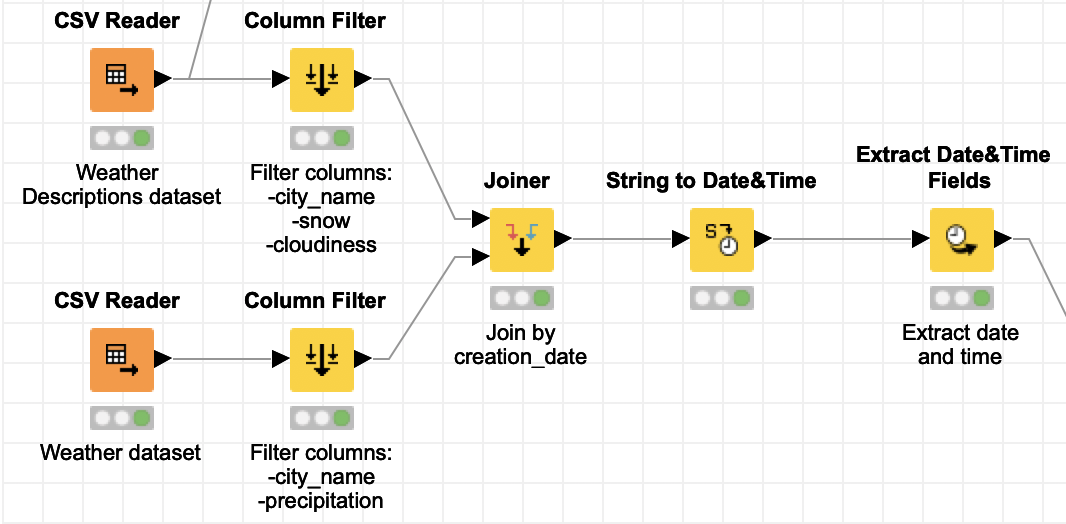
\includegraphics[width=10cm]{weather}
	\caption{Preparação dos \textit{datasets Weather\_Descriptions\_Braga} e \textit{Weather\_Braga}.}
\end{figure}

De seguida, procedeu-se à preparação do \textit{dataset Traffic\_Flow\_Braga}, procedendo-se à remoção das colunas \textit{city\_name} e \textit{road\_name}, seguida da extração da data e hora e agrupamento dos dados por \textit{road\_num}, hora, dia do mês e mês. De modo a juntar este \textit{dataset} ao obtido anteriormente, recorreu-se ao nodo \textit{Joiner}, unindo-se os \textit{datasets} por hora, dia do mês e mês, fazendo-se um \textit{Left Outer Join}.

\begin{figure}[H]
	\centering
	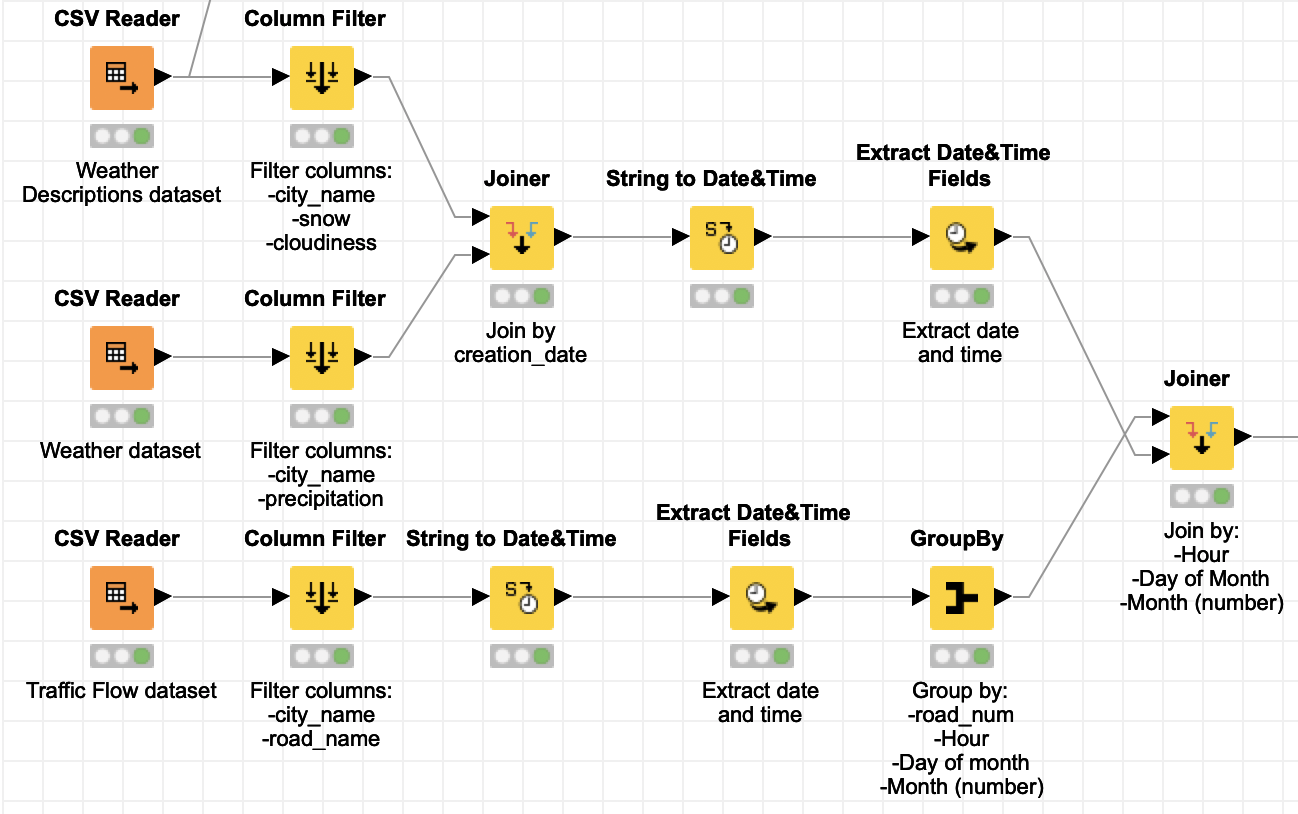
\includegraphics[width=10cm]{join}
	\caption{Preparação do \textit{dataset Traffic\_Flow\_Braga}.}
\end{figure}

Após a junção dos \textit{datasets}, eliminou-se a coluna \textit{creation\_date} e transformaram-se os valores "N/A", das colunas \textit{rain}, \textit{thunderstorm} e \textit{atmosphere}, em \textit{missing values}, recorrendo ao nodo \textit{String Manipulation}. De seguida, fez-se um \textit{merge} das colunas \textit{rain} e \textit{thunderstorm}, tendo-se alterado alguns dos valores ($"trovoada \ com \ chuva \ fraca" \rightarrow "chuva \ fraca"$, $"trovoada \ com \ chuva \ forte" \rightarrow "chuva \ forte"$ e $"trovoada" \rightarrow "chuva"$), tendo-se removido, no final, a coluna \textit{thunderstorm}. Por fim, com os valores da coluna \textit{clouds} construíram-se 6 intervalos:

\begin{enumerate}
	\item céu claro: $]-\inf,17[$;
	\item céu pouco nublado: $[17,34[$;
	\item nuvens dispersas: $[34,51[$;
	\item nuvens quebradas: $[51,68[$;
	\item nublado: $[68,85[$;
	\item muito nublado: $[85,+\inf[$;
\end{enumerate}

Tendo-se, de seguida, eliminado as colunas \textit{sunrise}, \textit{sunset} e \textit{clouds}.

\begin{figure}[H]
	\centering
	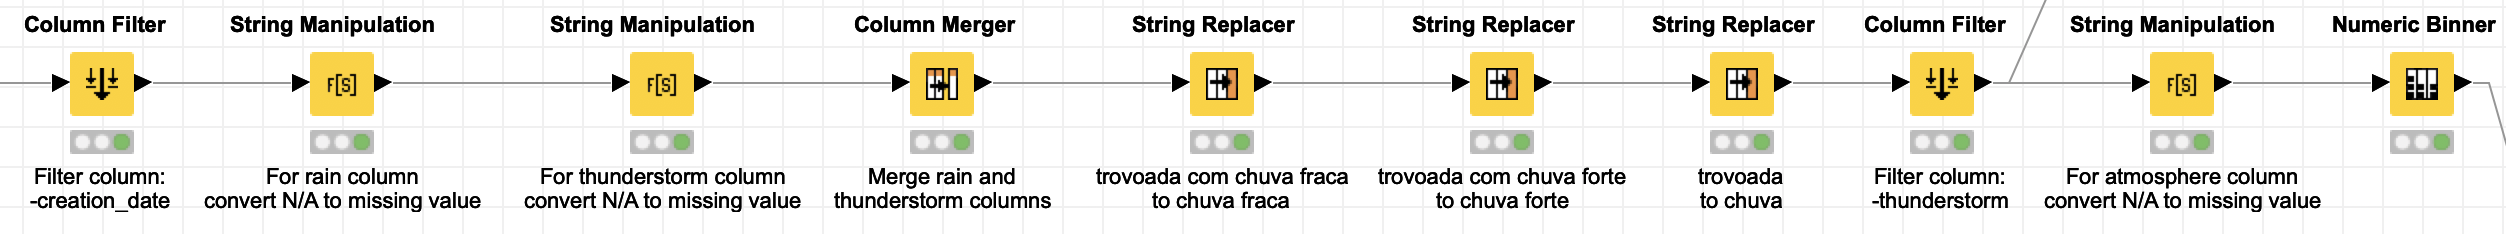
\includegraphics[width=15cm]{prep}
	\caption{Preparação dos dados.}
\end{figure}

Por fim, tratou-se o \textit{dataset} obtido após feito o tratamento do \textit{dataset Traffic\_Incidents}. Procedeu-se à extração do dia e da hora e removeram-se as colunas irrelevantes. Após tratado este \textit{dataset}, e recorrendo ao nodo \textit{Joiner}, uniu-se este \textit{dataset} com o obtido anteriormente por hora, dia do mês, mês e \textit{road\_num}. Deste modo, uniram-se os $4$ \textit{datasets} iniciais num único.

\begin{figure}[H]
	\centering
	\includegraphics[width=10cm]{Incident}
	\caption{Preparação do \textit{dataset} resultante do tratamento do \textit{dataset Traffic\_Incidents\_Braga}.}
\end{figure}

Após se ter apenas um \textit{dataset} eliminaram-se colunas que se acharam irrelevantes, servindo como apoio à decisão o nodo \textit{Rank Correlation}, e aos valores \textit{Undefined} da \textit{feature descriptions} atribui-se o valor \textit{Unknown Delay}, com o objetivo de diminuir a quantidade de atributos desta \textit{feature}.

De seguida, e tendo em conta que as colunas \textit{atmosphere} e \textit{rain} apresentam muitos \textit{missing values}, procedeu-se ao tratamento dos mesmos. 

Começou-se, então, por tratar os \textit{missing values} da coluna \textit{atmosphere}, tendo-se separado o \textit{dataset} em dois, recorrendo ao nodo \textit{Rule-based Row Splitter}. Um \textit{dataset} apresenta a coluna \textit{atmosphere} apenas com \textit{missing values} e o outro apresenta a coluna \textit{atmosphere} com os vários valores. De seguida, utilizaram-se \textit{Random Forest} para fazer a previsão dos \textit{missing values}, para isso, particionou-se o \textit{dataset} que apresentava os valores do atributo \textit{atmosphere}, tendo-se usado $80\%$ dos dados para treino. Após feita a previsão dos \textit{missing values}, procedeu-se à previsão dos \textit{missing values} do atributo \textit{rain}, tendo-se utilizado o mesmo raciocínio.

\begin{figure}[H]
	\centering
	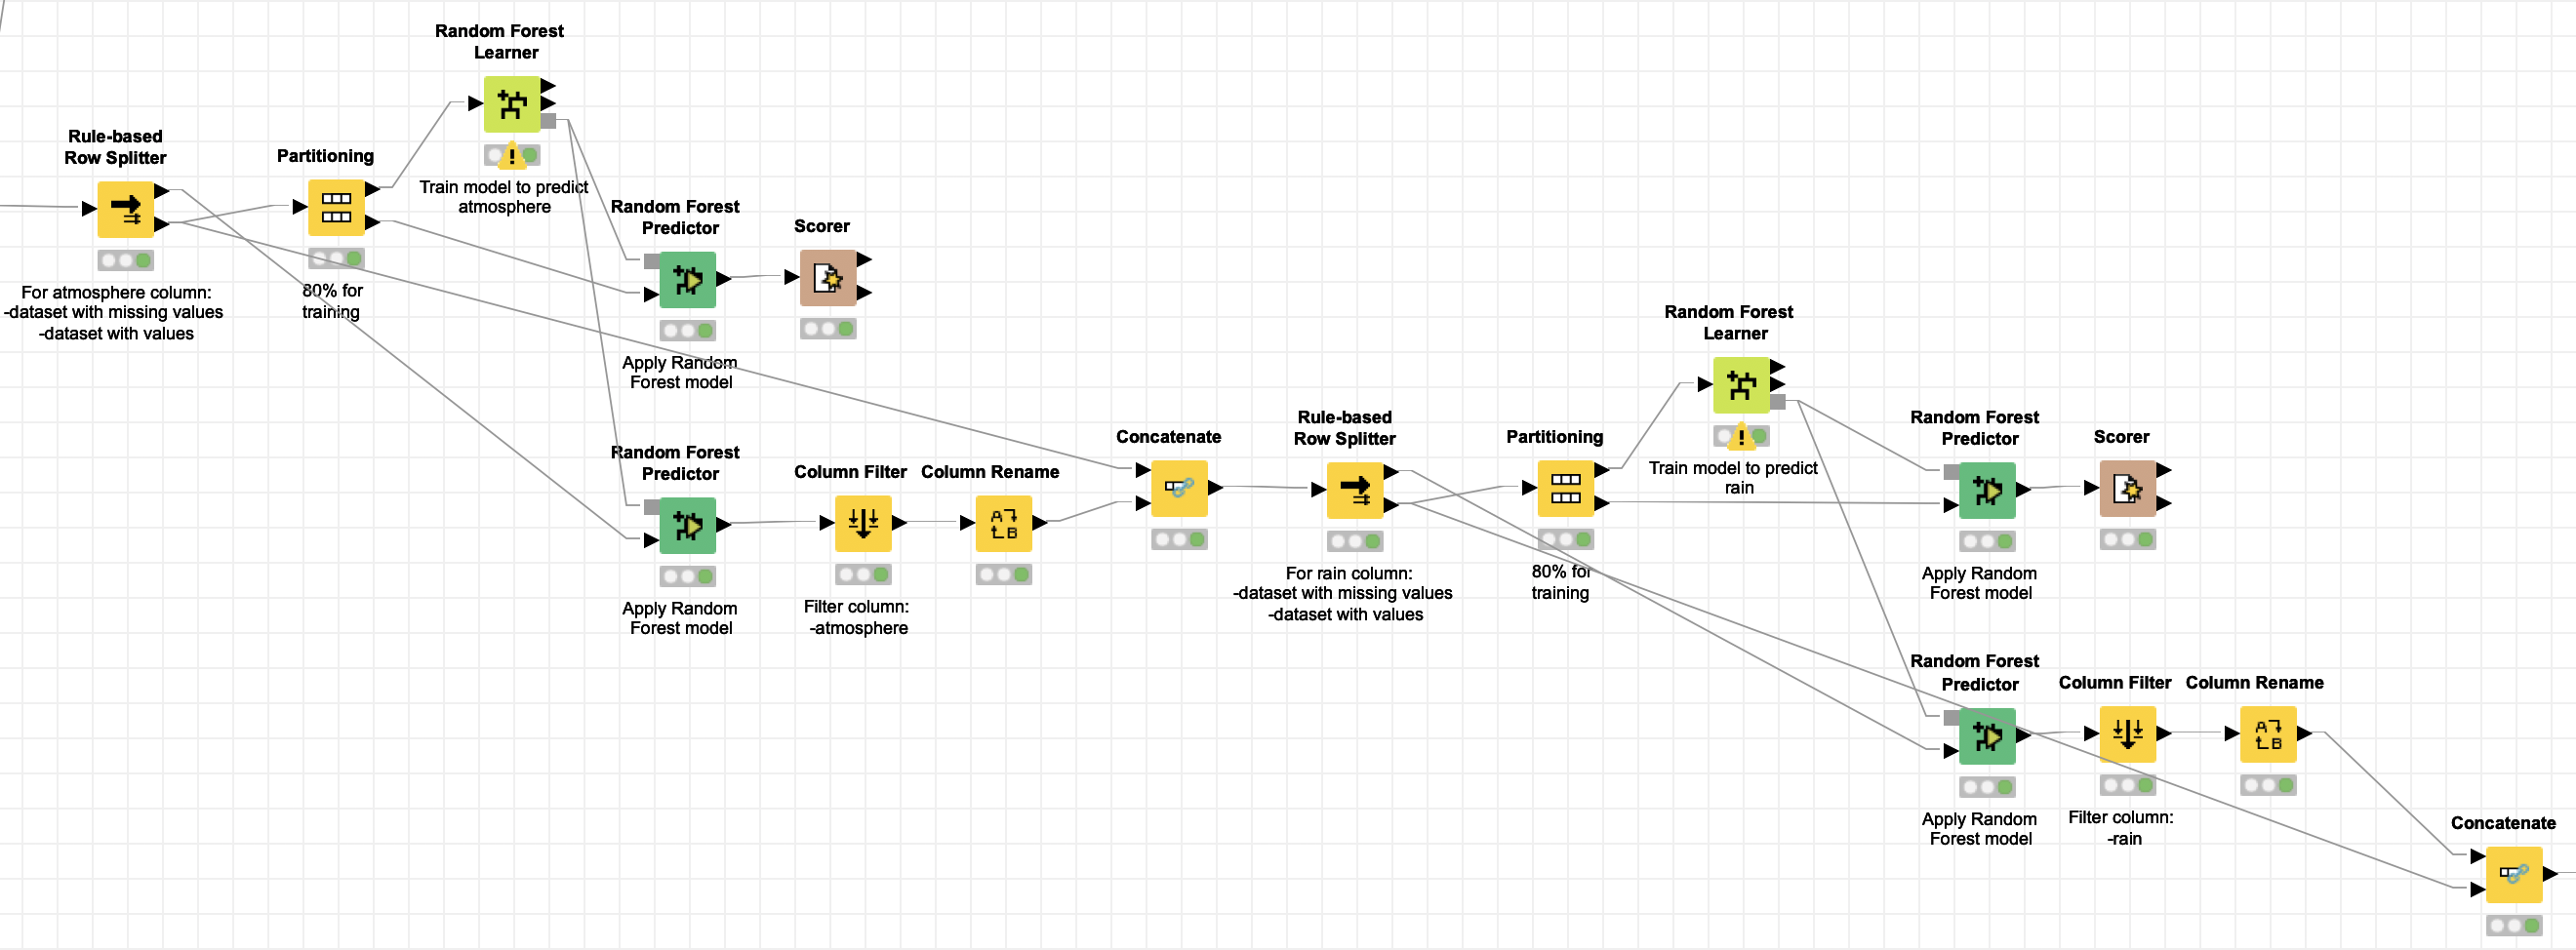
\includegraphics[width=15cm]{final}
	\caption{Previsão de \textit{missing values}.}
\end{figure}

Por fim, recorrendo ao nodo \textit{Duplicate Row Filter}, eliminaram-se linhas repetidas, efetuou-se o \textit{Label Encoding} dos valores que estavam em \textit{string} e trataram-se os \textit{missing values}, substituindo-os por um valor \textit{default}.

\begin{figure}[H]
	\centering
	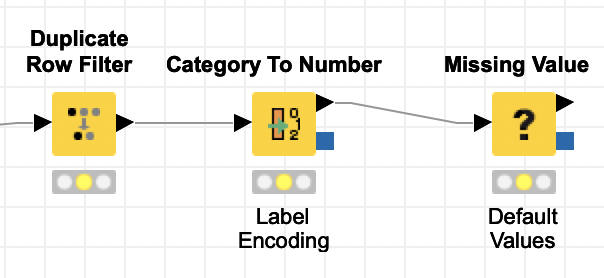
\includegraphics[width=5cm]{fim}
	\caption{Tratamento final.}
\end{figure}

Para finalizar o tratamento de dados foi ainda necessário perceber quais os dias que estavam com falta de dados, procedendo-se à eliminação destes, com o intuito de se ter um \textit{dataset} sem "buracos". Para isso, implementou-se o seguinte algoritmo:

\begin{lstlisting}[language=Python]
i=0
for i in range(1,13):
	for j in range(1,32):
	L=df[(df['Month (number)']==i)&(df['Day of month']==j)].dropna()
	L1=L[['Month (number)','Day of month','Hour','road_num']]
	L1 = L1.drop_duplicates()
	indexNames = df[(df['Month (number)']==i)&(df['Day of month']==j) ].index
	if len(L1)>96:
	if (len(L1)>=92 and len(L1)<96):
		i=i+1
	if len(L1)<96:
	try:
		df.drop(indexNames, inplace=True)
	except:
		pass
\end{lstlisting}

Após feito todo o tratamento acima mencionado, o \textit{dataset} está pronto para ser aplicado a uma rede que permita prever a \textit{feature speed\_diff}.


\end{document}
